\documentclass[11pt, a4paper]{article}\usepackage[]{graphicx}\usepackage[]{xcolor}
% maxwidth is the original width if it is less than linewidth
% otherwise use linewidth (to make sure the graphics do not exceed the margin)
\makeatletter
\def\maxwidth{ %
  \ifdim\Gin@nat@width>\linewidth
    \linewidth
  \else
    \Gin@nat@width
  \fi
}
\makeatother

\definecolor{fgcolor}{rgb}{0.345, 0.345, 0.345}
\newcommand{\hlnum}[1]{\textcolor[rgb]{0.686,0.059,0.569}{#1}}%
\newcommand{\hlsng}[1]{\textcolor[rgb]{0.192,0.494,0.8}{#1}}%
\newcommand{\hlcom}[1]{\textcolor[rgb]{0.678,0.584,0.686}{\textit{#1}}}%
\newcommand{\hlopt}[1]{\textcolor[rgb]{0,0,0}{#1}}%
\newcommand{\hldef}[1]{\textcolor[rgb]{0.345,0.345,0.345}{#1}}%
\newcommand{\hlkwa}[1]{\textcolor[rgb]{0.161,0.373,0.58}{\textbf{#1}}}%
\newcommand{\hlkwb}[1]{\textcolor[rgb]{0.69,0.353,0.396}{#1}}%
\newcommand{\hlkwc}[1]{\textcolor[rgb]{0.333,0.667,0.333}{#1}}%
\newcommand{\hlkwd}[1]{\textcolor[rgb]{0.737,0.353,0.396}{\textbf{#1}}}%
\let\hlipl\hlkwb

\usepackage{framed}
\makeatletter
\newenvironment{kframe}{%
 \def\at@end@of@kframe{}%
 \ifinner\ifhmode%
  \def\at@end@of@kframe{\end{minipage}}%
  \begin{minipage}{\columnwidth}%
 \fi\fi%
 \def\FrameCommand##1{\hskip\@totalleftmargin \hskip-\fboxsep
 \colorbox{shadecolor}{##1}\hskip-\fboxsep
     % There is no \\@totalrightmargin, so:
     \hskip-\linewidth \hskip-\@totalleftmargin \hskip\columnwidth}%
 \MakeFramed {\advance\hsize-\width
   \@totalleftmargin\z@ \linewidth\hsize
   \@setminipage}}%
 {\par\unskip\endMakeFramed%
 \at@end@of@kframe}
\makeatother

\definecolor{shadecolor}{rgb}{.97, .97, .97}
\definecolor{messagecolor}{rgb}{0, 0, 0}
\definecolor{warningcolor}{rgb}{1, 0, 1}
\definecolor{errorcolor}{rgb}{1, 0, 0}
\newenvironment{knitrout}{}{} % an empty environment to be redefined in TeX

\usepackage{alltt}

\usepackage[top = 0.8 in, bottom = 0.8 in, left = 1 in, right = 1 in ]{geometry}

\usepackage{amsmath, amssymb, amsfonts}
\usepackage{enumerate}
\usepackage{array}
\usepackage{multirow}
\usepackage{dingbat}
\usepackage{fontawesome5}
\usepackage{tasks}
\usepackage{bbding}
\usepackage{twemojis}
% how to use bull's eye ----- \scalebox{2.0}{\twemoji{bullseye}}
\usepackage{fontspec}
\usepackage{customdice}
% how to put dice face ------ \dice{2}

\title{MSMS 308 : Practical 01}
\author{Ananda Biswas}
\date{\today}

\newfontface\myfont{Myfont1-Regular.ttf}[LetterSpace=0.05em]
% how to use ---- {\setlength{\spaceskip}{1em plus 0.5em minus 0.5em} \fontsize{17}{20}\myfont --write text here-- \par}

\newfontface\cbfont{CaveatBrush-Regular.ttf}
% how to use --- \myfont --write text here--
\IfFileExists{upquote.sty}{\usepackage{upquote}}{}
\begin{document}

\maketitle


\section*{\faArrowAltCircleRight[regular] \textcolor{blue}{Question}}

\hspace{1cm} Consider the following survival data of 40 patients with myeloma. Compute and plot the estimated survival function, the probability density function, and the hazard function.
	
	\vspace{1cm}
	
	\begin{table}[!htbp]
	\def\arraystretch{1.5}
	
	\begin{center}
	\begin{tabular}{|>{\centering}m{4cm}|>{\centering}m{5cm}|>{\centering\arraybackslash}m{4cm}|}
	
	\hline
	
	Survival Time $t$ (months) & Number of Patients Surviving at Beginning of the Interval & Number of Patients Dying in the Interval \\
	
	\hline
	
	$0-5$ & 40 & 5 \\
	
	$5-10$ & 35 & 7 \\
	
	$10-15$ & 28 & 6 \\
	
	$15-20$ & 22 & 4 \\
	
	$20-25$ & 18 & 5 \\
	
	$25-30$ & 13 & 4 \\
	
	$30-35$ & 9 & 4 \\
	
	$35-40$ & 5 & 0 \\
	
	$40-45$ & 5 & 2 \\
	
	$45-50$ & 3 & 1 \\
	
	$\geq$ 50 & 2 & 2 \\
	
	\hline
	
	\end{tabular}
	\end{center}
	\end{table}




\section*{\faArrowAltCircleRight[regular] \textcolor{blue}{R Program, Plot and Interpretation}}

$$\widehat{S(t)} = \dfrac{\text{number of patients surviving longer than }t}{\text{total number of patients}}$$

$$\widehat{f(t)} = \dfrac{\text{number of patients dying in the interval beginning at time }t}{\text{(total number of patients )} \times \text{( interval width)}}$$

$$\widehat{h(t)} = \dfrac{\text{number of patients dying per unit time in the interval}}{(\text{number of patients surviving at }t) - \text{( number of deaths in the interval)}/2}$$

\newpage

\begin{knitrout}\tiny
\definecolor{shadecolor}{rgb}{0.969, 0.969, 0.969}\color{fgcolor}\begin{kframe}
\begin{alltt}
\hldef{survival_data} \hlkwb{<-} \hlkwd{read.csv}\hldef{(}\hlsng{'https://raw.githubusercontent.com/sakunisgithub/data_sets/refs/heads/master/msc_semester_3/life_time_prac_1.csv'}\hldef{,}
                          \hlkwc{stringsAsFactors} \hldef{=} \hlnum{TRUE}\hldef{)}
\end{alltt}
\end{kframe}
\end{knitrout}

\begin{knitrout}
\definecolor{shadecolor}{rgb}{0.969, 0.969, 0.969}\color{fgcolor}\begin{kframe}
\begin{alltt}
\hldef{total_number_of_patients} \hlkwb{<-} \hldef{survival_data}\hlopt{$}\hldef{no_at_risk[}\hlnum{1}\hldef{]}
\end{alltt}
\end{kframe}
\end{knitrout}

\begin{knitrout}
\definecolor{shadecolor}{rgb}{0.969, 0.969, 0.969}\color{fgcolor}\begin{kframe}
\begin{alltt}
\hldef{S_t_hat} \hlkwb{<-} \hldef{survival_data}\hlopt{$}\hldef{no_at_risk} \hlopt{/} \hldef{total_number_of_patients}
\end{alltt}
\end{kframe}
\end{knitrout}

\begin{knitrout}
\definecolor{shadecolor}{rgb}{0.969, 0.969, 0.969}\color{fgcolor}\begin{kframe}
\begin{alltt}
\hldef{interval_width} \hlkwb{<-} \hlnum{5}

\hldef{f_t_hat} \hlkwb{<-} \hldef{survival_data}\hlopt{$}\hldef{no_of_death} \hlopt{/} \hldef{(total_number_of_patients} \hlopt{*} \hldef{interval_width)}

\hldef{f_t_hat[}\hlkwd{length}\hldef{(f_t_hat)]} \hlkwb{=} \hlnum{NA}
\end{alltt}
\end{kframe}
\end{knitrout}

\begin{knitrout}
\definecolor{shadecolor}{rgb}{0.969, 0.969, 0.969}\color{fgcolor}\begin{kframe}
\begin{alltt}
\hlcom{# a = number_of_patients_dying_per_unit_time_in_the_interval}

\hldef{a} \hlkwb{<-} \hldef{survival_data}\hlopt{$}\hldef{no_of_death} \hlopt{/} \hldef{interval_width}

\hldef{h_t_hat} \hlkwb{<-} \hldef{a} \hlopt{/} \hldef{(survival_data}\hlopt{$}\hldef{no_at_risk} \hlopt{-} \hldef{survival_data}\hlopt{$}\hldef{no_of_death} \hlopt{/} \hlnum{2}\hldef{)}

\hldef{h_t_hat[}\hlkwd{length}\hldef{(h_t_hat)]} \hlkwb{=} \hlnum{NA}
\end{alltt}
\end{kframe}
\end{knitrout}

\begin{knitrout}
\definecolor{shadecolor}{rgb}{0.969, 0.969, 0.969}\color{fgcolor}\begin{kframe}
\begin{alltt}
\hldef{analysis_table} \hlkwb{<-} \hlkwd{data.frame}\hldef{(survival_data,}
                             \hlkwc{t} \hldef{= (}\hlnum{0}\hlopt{:}\hlnum{10}\hldef{)}\hlopt{*}\hlnum{5}\hldef{,}
                             \hlkwc{S_t_hat} \hldef{=} \hlkwd{round}\hldef{(S_t_hat,} \hlkwc{digits} \hldef{=} \hlnum{3}\hldef{),}
                             \hlkwc{f_t_hat} \hldef{=} \hlkwd{round}\hldef{(f_t_hat,} \hlkwc{digits} \hldef{=} \hlnum{3}\hldef{),}
                             \hlkwc{h_t_hat} \hldef{=} \hlkwd{round}\hldef{(h_t_hat,} \hlkwc{digits} \hldef{=} \hlnum{3}\hldef{))}
\end{alltt}
\end{kframe}
\end{knitrout}

\begin{knitrout}
\definecolor{shadecolor}{rgb}{0.969, 0.969, 0.969}\color{fgcolor}\begin{kframe}
\begin{alltt}
\hldef{analysis_table}
\end{alltt}
\begin{verbatim}
##    survival_time no_at_risk no_of_death  t S_t_hat f_t_hat h_t_hat
## 1           0--5         40           5  0   1.000   0.025   0.027
## 2          5--10         35           7  5   0.875   0.035   0.044
## 3         10--15         28           6 10   0.700   0.030   0.048
## 4         15--20         22           4 15   0.550   0.020   0.040
## 5         20--25         18           5 20   0.450   0.025   0.065
## 6         25--30         13           4 25   0.325   0.020   0.073
## 7         30--35          9           4 30   0.225   0.020   0.114
## 8         35--40          5           0 35   0.125   0.000   0.000
## 9         40--45          5           2 40   0.125   0.010   0.100
## 10        45--50          3           1 45   0.075   0.005   0.080
## 11          >=50          2           2 50   0.050      NA      NA
\end{verbatim}
\end{kframe}
\end{knitrout}



\newpage

\begin{knitrout}
\definecolor{shadecolor}{rgb}{0.969, 0.969, 0.969}\color{fgcolor}\begin{kframe}
\begin{alltt}
\hldef{t_last} \hlkwb{<-} \hlkwd{max}\hldef{(analysis_table}\hlopt{$}\hldef{t)}

\hldef{S_t_hat_last} \hlkwb{<-} \hldef{analysis_table} \hlopt \hlkwd{filter}\hldef{(t} \hlopt{==} \hldef{t_last)} \hlopt \hlkwd{pull}\hldef{(S_t_hat)}

\hldef{analysis_table} \hlopt
  \hlkwd{ggplot}\hldef{(}\hlkwd{aes}\hldef{(}\hlkwc{x} \hldef{= t,} \hlkwc{y} \hldef{= S_t_hat))} \hlopt{+}
  \hlkwd{geom_step}\hldef{(}\hlkwc{direction} \hldef{=} \hlsng{"hv"}\hldef{,} \hlkwc{linewidth} \hldef{=} \hlnum{1}\hldef{,} \hlkwc{color} \hldef{=} \hlsng{"blue"}\hldef{)} \hlopt{+}
  \hlkwd{geom_point}\hldef{(}\hlkwc{size} \hldef{=} \hlnum{2}\hldef{,} \hlkwc{color} \hldef{=} \hlsng{"red"}\hldef{,} \hlkwc{shape} \hldef{=} \hlnum{4}\hldef{,} \hlkwc{stroke} \hldef{=} \hlnum{2}\hldef{)} \hlopt{+}
  \hlkwd{annotate}\hldef{(}\hlsng{"segment"}\hldef{,} \hlkwc{x} \hldef{= t_last,} \hlkwc{xend} \hldef{= t_last} \hlopt{+} \hlnum{5}\hldef{,}
           \hlkwc{y} \hldef{= S_t_hat_last,} \hlkwc{yend} \hldef{= S_t_hat_last,} \hlkwc{color} \hldef{=} \hlsng{"blue"}\hldef{,} \hlkwc{linewidth} \hldef{=} \hlnum{1}\hldef{)} \hlopt{+}
  \hlkwd{scale_x_continuous}\hldef{(}\hlkwc{limits} \hldef{=} \hlkwd{c}\hldef{(}\hlnum{0}\hldef{,} \hlnum{55}\hldef{),} \hlkwc{breaks} \hldef{=} \hlkwd{seq}\hldef{(}\hlnum{0}\hldef{,} \hlnum{55}\hldef{,} \hlnum{5}\hldef{))} \hlopt{+}
  \hlkwd{labs}\hldef{(}\hlkwc{x} \hldef{=} \hlsng{"t (months)"}\hldef{,}
       \hlkwc{y} \hldef{=} \hlsng{"Estimated Survival Function"}\hldef{,}
       \hlkwc{title} \hldef{=} \hlsng{"Plot of Estimated Survival Function"}\hldef{)}
\end{alltt}
\end{kframe}
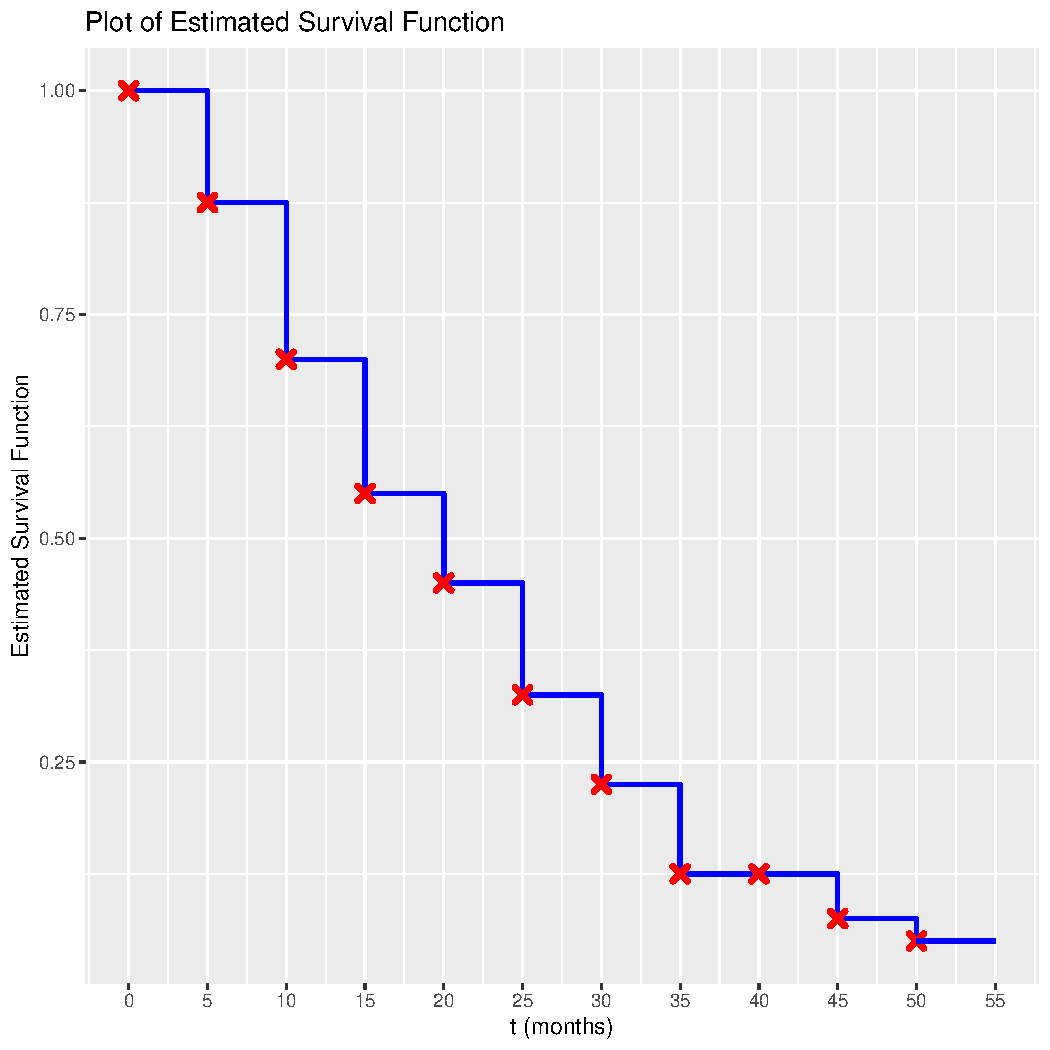
\includegraphics[width=\maxwidth]{figure/unnamed-chunk-9-1} 
\end{knitrout}

\smallpencil \hspace{0.1cm} {\setlength{\spaceskip}{1em plus 0.5em minus 0.5em} \fontsize{17}{20}\myfont The median survival time for myeloma patients is approximately 17.5 months. \par}

\newpage

\begin{knitrout}
\definecolor{shadecolor}{rgb}{0.969, 0.969, 0.969}\color{fgcolor}\begin{kframe}
\begin{alltt}
\hldef{t_first} \hlkwb{<-} \hlkwd{min}\hldef{(analysis_table}\hlopt{$}\hldef{t)}

\hldef{f_t_hat_first} \hlkwb{<-} \hldef{analysis_table} \hlopt \hlkwd{filter}\hldef{(t} \hlopt{==} \hldef{t_first)} \hlopt \hlkwd{pull}\hldef{(f_t_hat)}

\hldef{analysis_table[}\hlopt{-}\hlkwd{dim}\hldef{(analysis_table)[}\hlnum{1}\hldef{],]} \hlopt
  \hlkwd{ggplot}\hldef{(}\hlkwd{aes}\hldef{(}\hlkwc{x} \hldef{= t}\hlopt{+}\hlnum{2.5}\hldef{,} \hlkwc{y} \hldef{= f_t_hat))} \hlopt{+}
  \hlkwd{geom_line}\hldef{(}\hlkwc{linewidth} \hldef{=} \hlnum{1}\hldef{,} \hlkwc{col} \hldef{=} \hlsng{"blue"}\hldef{)} \hlopt{+}
  \hlkwd{geom_point}\hldef{(}\hlkwc{size} \hldef{=} \hlnum{2}\hldef{,} \hlkwc{col} \hldef{=} \hlsng{"red"}\hldef{,} \hlkwc{shape} \hldef{=} \hlnum{4}\hldef{,} \hlkwc{stroke} \hldef{=} \hlnum{2}\hldef{)} \hlopt{+}
  \hlkwd{annotate}\hldef{(}\hlsng{"segment"}\hldef{,} \hlkwc{x} \hldef{= t_first,} \hlkwc{xend} \hldef{= t_first} \hlopt{+} \hlnum{2.5}\hldef{,}
           \hlkwc{y} \hldef{=} \hlnum{0}\hldef{,} \hlkwc{yend} \hldef{= f_t_hat_first,} \hlkwc{color} \hldef{=} \hlsng{"blue"}\hldef{,} \hlkwc{linewidth} \hldef{=} \hlnum{1}\hldef{)} \hlopt{+}
  \hlkwd{scale_x_continuous}\hldef{(}\hlkwc{limits} \hldef{=} \hlkwd{c}\hldef{(}\hlnum{0}\hldef{,} \hlnum{50}\hldef{),} \hlkwc{breaks} \hldef{=} \hlkwd{seq}\hldef{(}\hlnum{0}\hldef{,} \hlnum{50}\hldef{,} \hlnum{5}\hldef{))} \hlopt{+}
  \hlkwd{labs}\hldef{(}\hlkwc{x} \hldef{=} \hlsng{"t (months)"}\hldef{,}
       \hlkwc{y} \hldef{=} \hlsng{"Estimated Density Function"}\hldef{,}
       \hlkwc{title} \hldef{=} \hlsng{"Plot of Estimated Density Function"}\hldef{)}
\end{alltt}
\end{kframe}
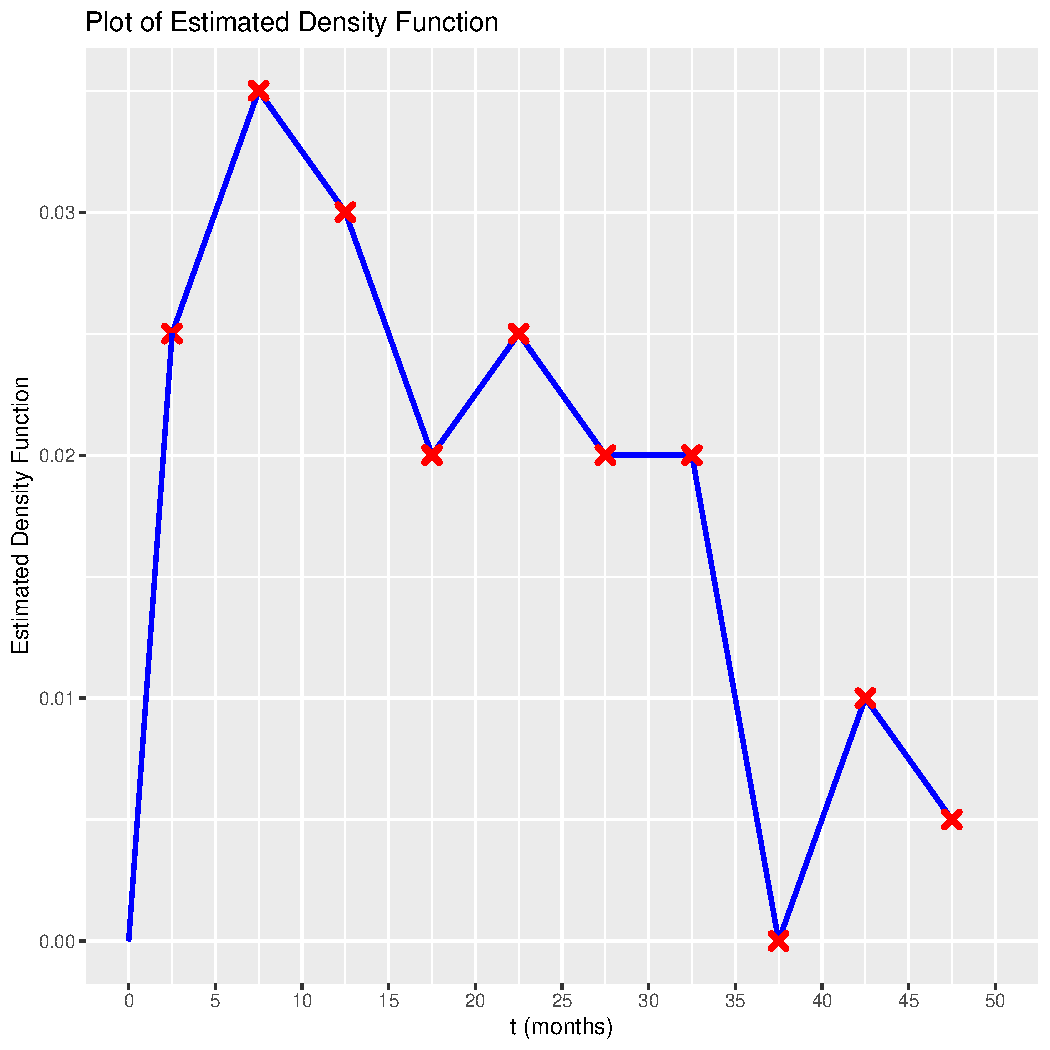
\includegraphics[width=\maxwidth]{figure/unnamed-chunk-10-1} 
\end{knitrout}

\smallpencil \hspace{0.1cm} {\setlength{\spaceskip}{1em plus 0.5em minus 0.5em} \fontsize{17}{20}\myfont Death due to myeloma is most likely occur in 5 to 10 months. \par}

\newpage

\begin{knitrout}
\definecolor{shadecolor}{rgb}{0.969, 0.969, 0.969}\color{fgcolor}\begin{kframe}
\begin{alltt}
\hldef{h_t_hat_first} \hlkwb{=} \hldef{analysis_table} \hlopt \hlkwd{filter}\hldef{(t} \hlopt{==} \hldef{t_first)} \hlopt \hlkwd{pull}\hldef{(h_t_hat)}

\hldef{analysis_table[}\hlopt{-}\hlkwd{dim}\hldef{(analysis_table)[}\hlnum{1}\hldef{],]} \hlopt
  \hlkwd{ggplot}\hldef{(}\hlkwd{aes}\hldef{(}\hlkwc{x} \hldef{= t}\hlopt{+}\hlnum{2.5}\hldef{,} \hlkwc{y} \hldef{= h_t_hat))} \hlopt{+}
  \hlkwd{geom_line}\hldef{(}\hlkwc{linewidth} \hldef{=} \hlnum{1}\hldef{,} \hlkwc{col} \hldef{=} \hlsng{"blue"}\hldef{)} \hlopt{+}
  \hlkwd{geom_point}\hldef{(}\hlkwc{size} \hldef{=} \hlnum{2}\hldef{,} \hlkwc{col} \hldef{=} \hlsng{"red"}\hldef{,} \hlkwc{shape} \hldef{=} \hlnum{4}\hldef{,} \hlkwc{stroke} \hldef{=} \hlnum{2}\hldef{)} \hlopt{+}
  \hlkwd{annotate}\hldef{(}\hlsng{"segment"}\hldef{,} \hlkwc{x} \hldef{=} \hlnum{0}\hldef{,} \hlkwc{xend} \hldef{= h_t_hat_first} \hlopt{+} \hlnum{2.5}\hldef{,}
           \hlkwc{y} \hldef{=} \hlnum{0}\hldef{,} \hlkwc{yend} \hldef{= h_t_hat_first,} \hlkwc{color} \hldef{=} \hlsng{"blue"}\hldef{,} \hlkwc{linewidth} \hldef{=} \hlnum{1}\hldef{)} \hlopt{+}
  \hlkwd{scale_x_continuous}\hldef{(}\hlkwc{limits} \hldef{=} \hlkwd{c}\hldef{(}\hlnum{0}\hldef{,} \hlnum{50}\hldef{),} \hlkwc{breaks} \hldef{=} \hlkwd{seq}\hldef{(}\hlnum{0}\hldef{,} \hlnum{50}\hldef{,} \hlnum{5}\hldef{))} \hlopt{+}
  \hlkwd{labs}\hldef{(}\hlkwc{x} \hldef{=} \hlsng{"t (months)"}\hldef{,}
       \hlkwc{y} \hldef{=} \hlsng{"Estimated Hazard Function"}\hldef{,}
       \hlkwc{title} \hldef{=} \hlsng{"Plot of Estimated Hazard Function"}\hldef{)}
\end{alltt}
\end{kframe}
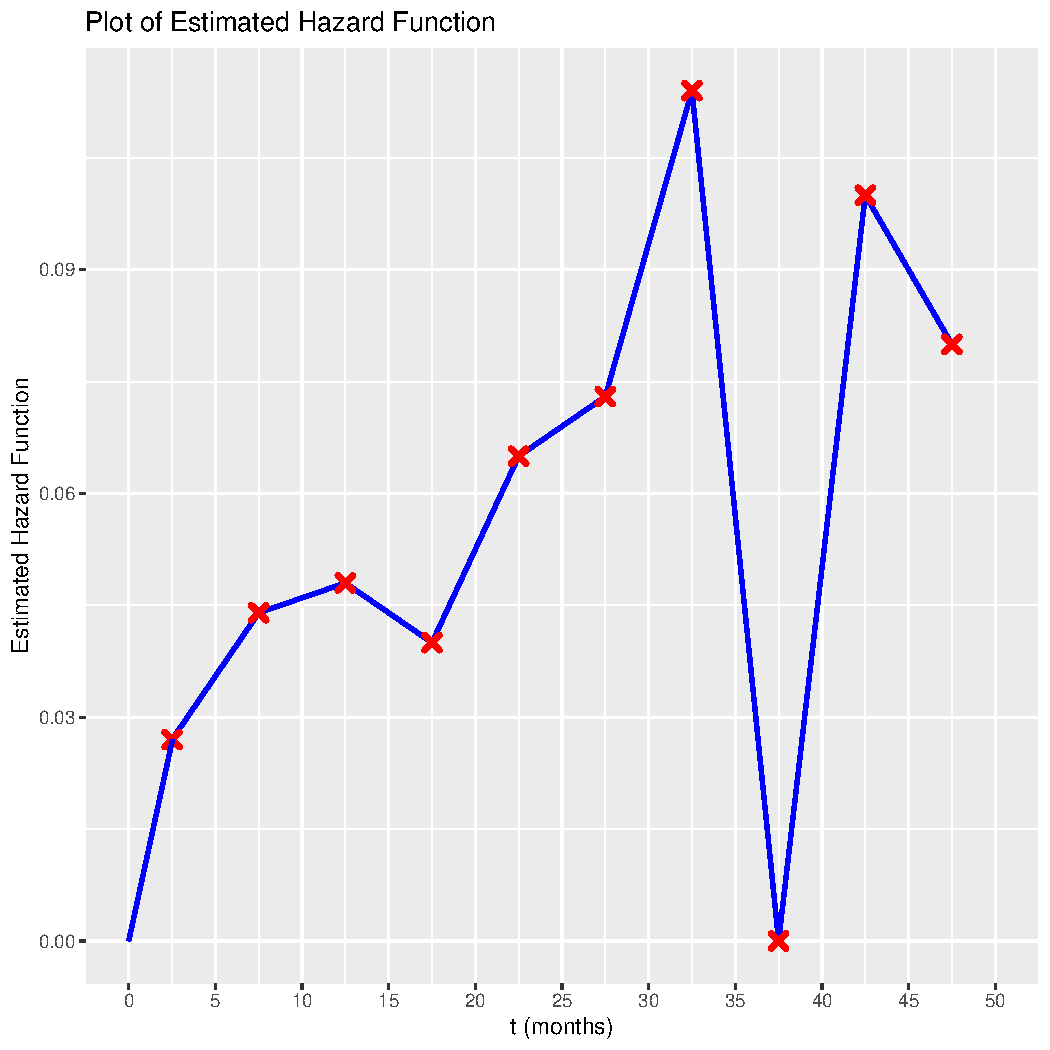
\includegraphics[width=\maxwidth]{figure/unnamed-chunk-11-1} 
\end{knitrout}

\smallpencil \hspace{0.1cm} {\setlength{\spaceskip}{1em plus 0.5em minus 0.5em} \fontsize{17}{20}\myfont The hazard function shows an increasing trend and reaches its peak in 30 to 35 months, so risk of death increases over time. \par}

\end{document}
